We perform the projection in Eq. \eqref{eq:y_projection} for a regularization of
the form $\vf{R} = \text{diag}([R_t, R_t, R_n])$. For simplicity, we drop
contact subindex $i$. We make the change of variables
$\tilde{\bgamma}=\vf{R}^{1/2}\bgamma$ and $\tilde{\vf{y}}=\vf{R}^{1/2}\vf{y}$
\cite{bib:todorov2014}, and observe that $\tilde{\bgamma}$ is the Euclidian
projection of $\tilde{\vf{y}}$ onto cone $\tilde{\mathcal{F}}$ with coefficient
$\tilde \mu =\mu\,(R_t/R_n)^{1/2}$. We conclude that
\begin{eqnarray*}
  P_\mathcal{F}(\vf{y})=\vf{R}^{-1/2} P_{\tilde{\mathcal{F}}}(\tilde{\vf{y}}),
\end{eqnarray*}

We partition $\mathbb{R}^3$ into three regions, see Fig.~
\ref{fig:cone_regions}: closed cone $\tilde{\mathcal{F}}$, denoted with
$\mathcal{R}_I$, the interior of the polar $\tilde{\mathcal{F}}^\circ$, denoted
with $\mathcal{R}_{III}$, and the remaining area, which we denote with
$\mathcal{R}_{II}$. For $\tilde{\vf{y}}\in\mathcal{R}_I$ we simply have that
$P_{\tilde{\mathcal{F}}}(\tilde{\vf{y}}) = \tilde{\vf{y}}$. When
$\tilde{\vf{y}}\in\mathcal{R}_{III}$, $P_{\tilde{\mathcal{F}}}(\tilde{\vf{y}}) =
\vf{0}$. Finally, when $\tilde{\vf{y}}\in\mathcal{R}_{II}$, we evaluate
$P_{\tilde{\mathcal{F}}}(\tilde{\vf{y}})$ via Euclidean projection onto the
boundary of $\tilde{\mathcal{F}}$, which admits a simple formula. We define
$\hat{\vf{f}}=[\tilde{\mu}\hat{\vf{t}}, 1]/\sqrt{1+\tilde{\mu}^2}$, the unit
vector along the wall of the cone shown in Fig.~\ref{fig:cone_regions}, with
$\hat{\vf{t}}=\tilde{\vf{y}}_t/\Vert\tilde{\vf{y}}_t\Vert=\vf{y}_t/\Vert\vf{y}_t\Vert$.
Then the projection is computed as
$\tilde{\bgamma}=(\tilde{\vf{y}}\cdot\hat{\vf{f}})\hat{\vf{f}}$. After some
algebraic manipulation we have that $P_{\tilde{\mathcal{F}}}(\tilde{\vf{y}}) =
[\tilde{\bgamma}_t, \tilde{\gamma}_n]$ with
\begin{align*}
  \tilde{\bgamma}_t       &= \tilde{\mu}\tilde{\gamma}_n\hat{\vf{t}},\\
        \tilde{\gamma}_n  &= \frac{1}{1+\tilde{\mu}^2}\left(\tilde{y}_n +
	\tilde{\mu}\tilde{y}_r\right),
\end{align*}
where $\tilde{y}_r=\Vert\tilde{\vf{y}}_t\Vert$. Note that this formula is
well-defined on $\mathcal{R}_{II}$, since $\vf{y}_t = \vf{0}$ only if $\vf{y}$ is in regions $\mathcal{R}_{I}$ or $\mathcal{R}_{III}$.
\begin{figure}[!h]
    \centering
    %\vspace{6pt}
    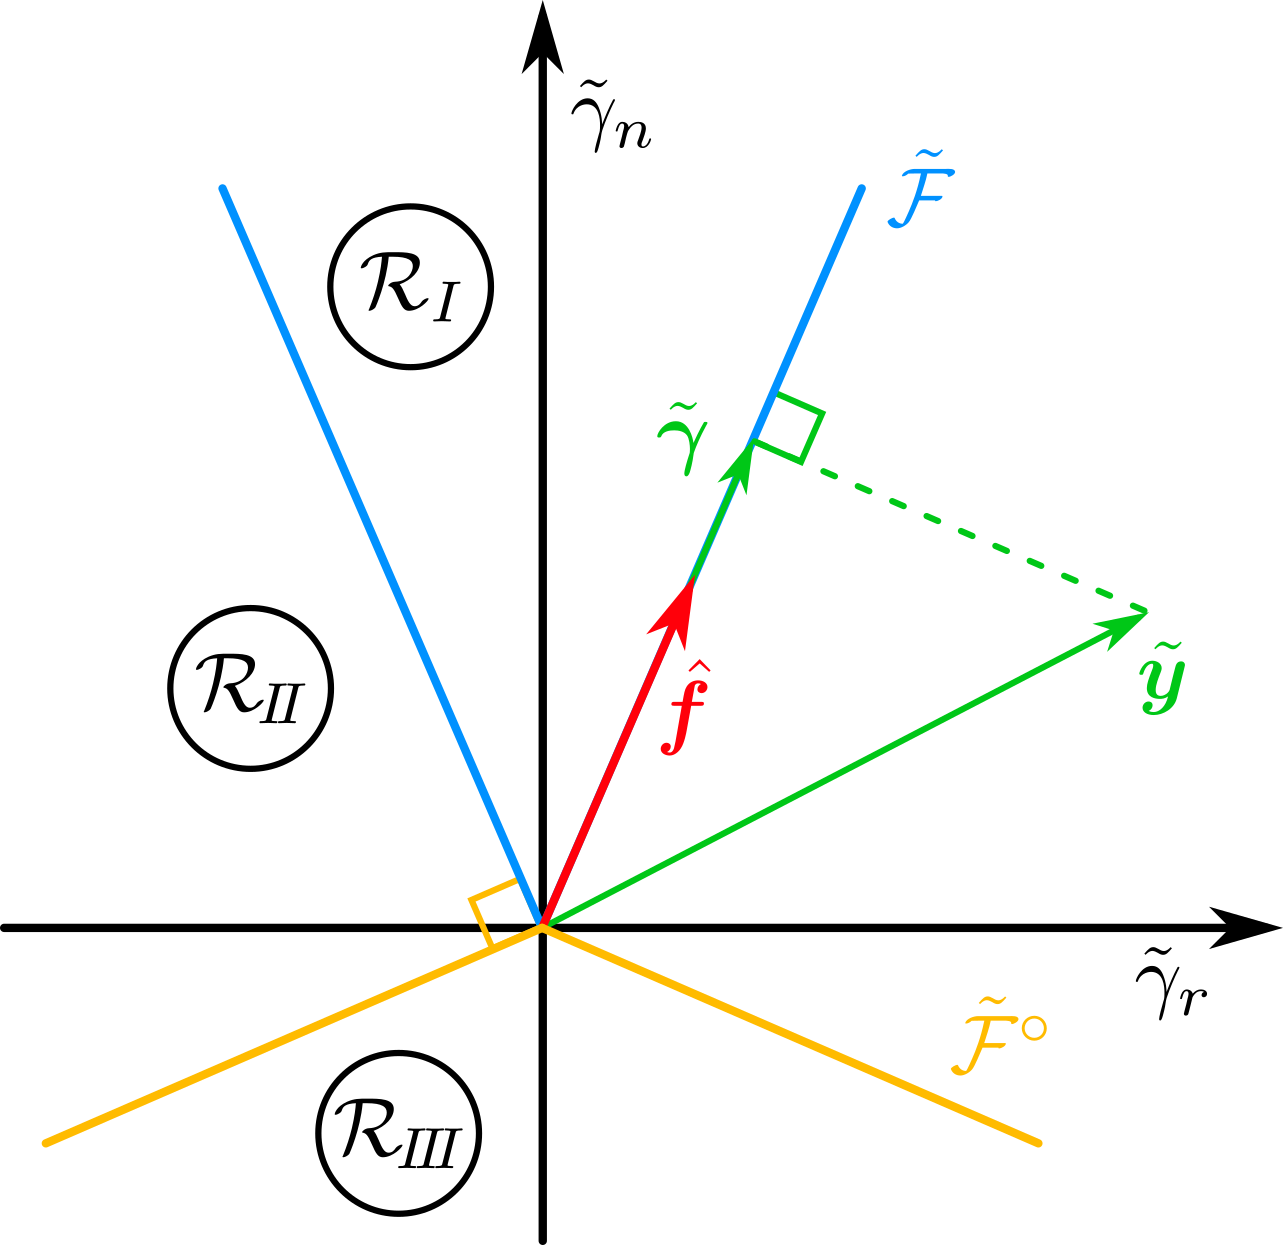
\includegraphics[width=0.6\columnwidth]{figures/schematics/analytical_inverse_dynamics.png}
    \caption{Geometry of the projection and regions in the
    $\tilde{\vf{y}}$ space.}
    \label{fig:cone_regions}
\end{figure}

Finally, we apply the inverse transformation
$\bgamma=\mf{R}^{-1/2}P_{\tilde{\mathcal{F}}}(\tilde{\vf{y}})$ and after some
algebraic manipulation we recover the projection $\bgamma =
P_\mathcal{F}(\vf{y})$ in Eq. \eqref{eq:analytical_y_projection}.


